%\hspace{24pt}
%In this section, we introduce SDN architecture and existing load balancing techniques. 
%In order to balance the total AP load, various association control schemes have been proposed in the past.


% ====remove SDN section by little six====
% \subsection{Software Defined Network}
% SDN\cite{mckeown2008openflow} is the key enabler in the new networking architecture innovation, which makes packet forwarding become more flexible and easy-management. It decouples the forwarding and control planes of switches, which means that the sets of forwarding rules in switches can be defined in any way, and the network control is all conducted by SDN controller to have total network view. This revolution allows network administrator to design network experimentation over production and academic network. Figure \ref{fig:SDN-Architecture} shows the architecture of SDN.

%% Fig2.1
% \begin{figure}[tbp]
% \begin{center}
% 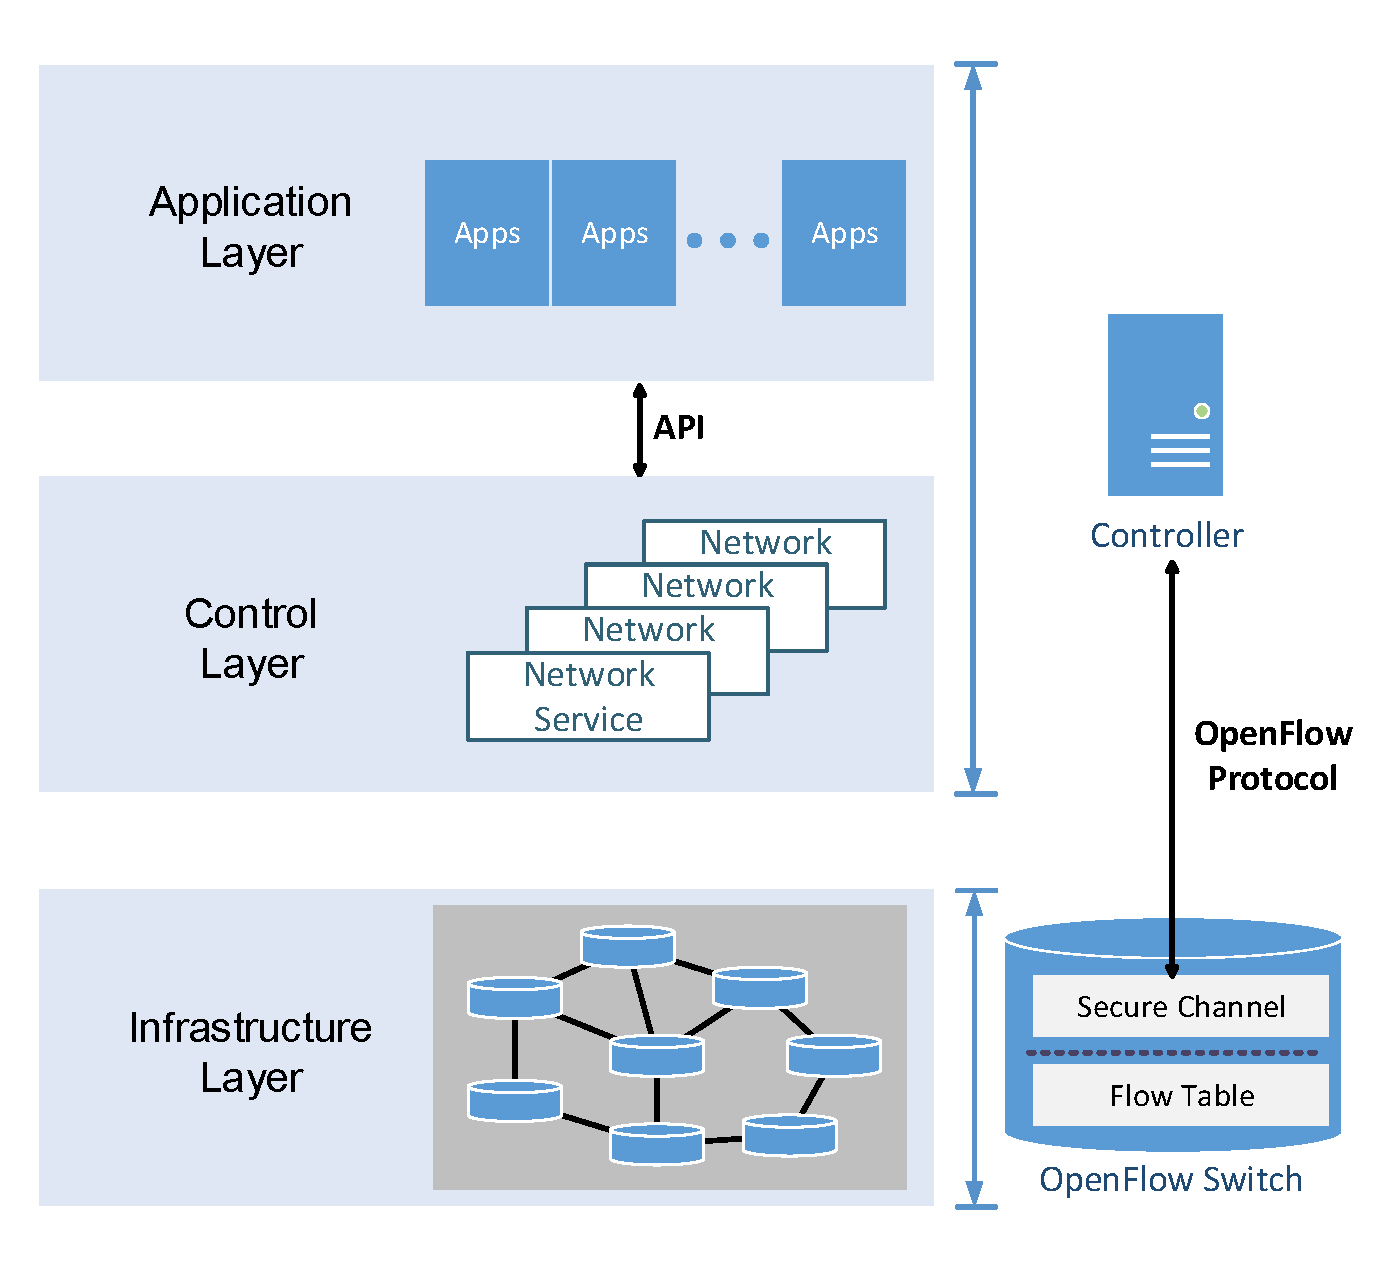
\includegraphics[width=3.4in]{images/SDN_architecture.pdf}
% \end{center}
% \caption{SDN Architecture}
% \label{fig:SDN-Architecture}
% \end{figure}
%\clearpage

% The Stanford University proposed a wireless SDN platform in Clean Slate plan, called “OpenRoads” \cite{yap2010openroads}. It is built on OpenFlow and SNMP, so it allows researchers to design mobility management mechanism by changing the forwarding rule or controlling the wireless AP configurations. For example in \cite{kim2014seamless} and \cite{dely2013software}, the issues of handover and performance anomaly are discussed based on SDN. The approach of OpenRoads project shows that continued innovation and development in wireless SDN can be expected.



% \subsection{Association Control}
%In this section, we introduce some existing user-to-AP association decision schemes which were proposed to balance the total AP load. 
In this section, we describe existing association control schemes and load balancing schemes in literature.
% which are based on association control.
%We classify these schemes into three categories: \emph{strongest signal first} (SSF), \emph{least load first} (LLF) and \emph{Cell Breathing}.

%\begin{itemize}
%	\item SSF: 
The strongest signal first (SSF) method is the traditional association mechanism defined in IEEE 802.11 standards~\cite{ieee2001ieee}. 
	%If a user has many APs to choose, it will select the AP with the largest Received Signal Strength Indicator (RSSI) value to associate with.
%	When a device detects more than one AP
The device selects the AP with the largest received signal strength indicator (RSSI) value for association.
%	In \cite{teng2009d} and \cite{wu2007proactive}, user are setting to re-associated with the stronger signal strength AP. 
This method is also widely adopted in handoff schemes~\cite{teng2009d,wu2007proactive}.
%	The main problem of these schemes is the load imbalance of APs. 
%	When too many users associate to an AP with strong signal at the same time, these users may incur worse performance from the overloaded AP.
	
%	\item LLF: 
Least load first (LLF) is the most straightforward load balancing scheme, where users select the  AP with least number of users~\cite{papanikos2001study}.
	% proposed an association metrics by considering the number of users currently associated with AP. 
In~\cite{balachandran2002hot},  
	%Balachandran et al. proposed an association selection scheme that 
users associate to the AP which 
	%can provide sufficient bandwidth based on the 
	can meet users' bandwidth requirements. 
In \cite{bejerano2004fairness}, 
	%Bejerano et al. further consider 
	the fairness among all users in association control is considered.

%	\item $\emph{Cell Breathing}$: 
The cell breathing concept has been studied mostly in code devision multiple access (CDMA) cellular network. 
In \cite{bahl2007cell} and \cite{bejerano2009cell}, cell breathing was applied to IEEE 802.11 WLANs. 
Figure \ref{fig:cell-breathing} illustrates an example of cell breathing method. 
First, the three APs in Figure~\ref{fig:fig2_2a} are associated with 1, 7, and 1 users, respectively.
Through adjusting the power levels of APs, some users of AP b shift to adjacent APs, and then the APs are all associated with three users in Figure \ref{fig:fig2_2b}. 
In the cell breathing method, %an access controller can obtain the load of APs, but 
without the information of users' positions, 
%In this case, 
the controller can only adjust the beacon power of the APs with the highest load step by step until the load of APs is balanced.
%For the related work of cell breathing method, 
%To achieve load balancing, 
%in \cite{bejerano2009cell}, Bejerano et al. proposed an algorithm to 
%\cite{bejerano2009cell} determines globally optimal inter-AP fairness. 
%However, both \cite{bahl2007cell} and \cite{bejerano2009cell} 
%adjust the AP power level based on limited information (e.g., number of users).
%cannot adjust the AP power level adaptively due to limited information of AP loads. 
% without any prediction of association change trend.
%\end{itemize}

%% Fig:2.2
\begin{figure}
	\centering
		\subfigure[All APs have the same power level.]
		{
			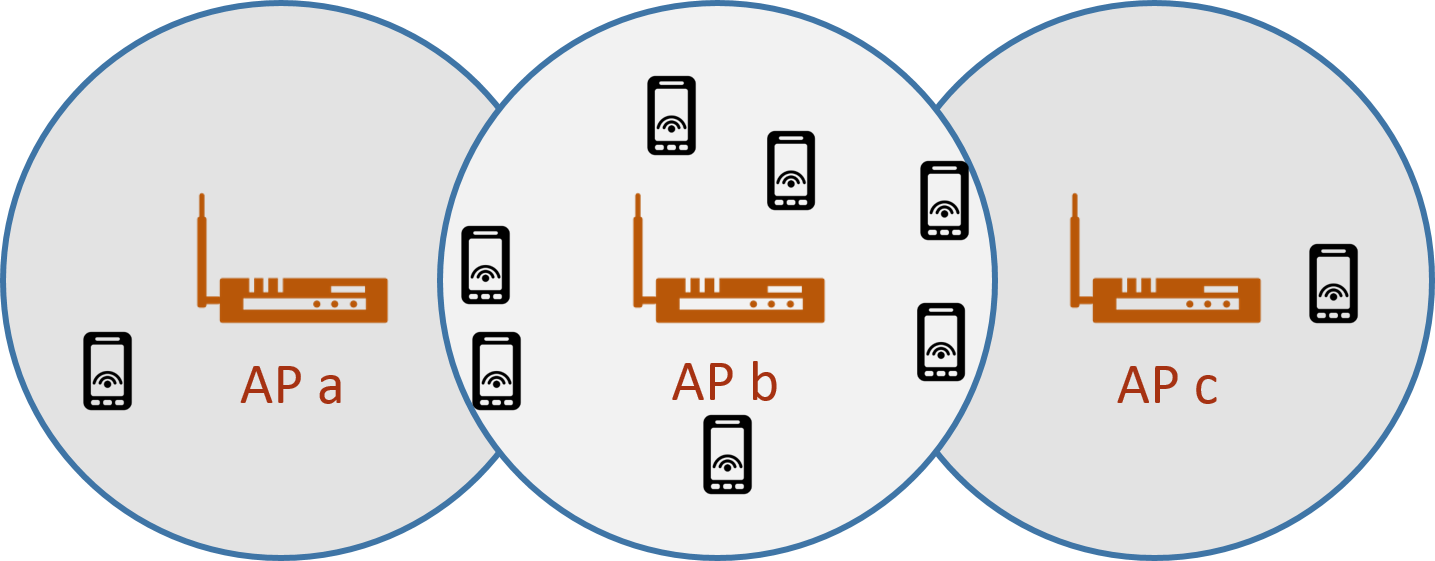
\includegraphics[scale=0.23]{images/cb_before.png}
			\label{fig:fig2_2a}
		}
		\subfigure[ AP $b$ transmits with the lowest power level.]
		{
			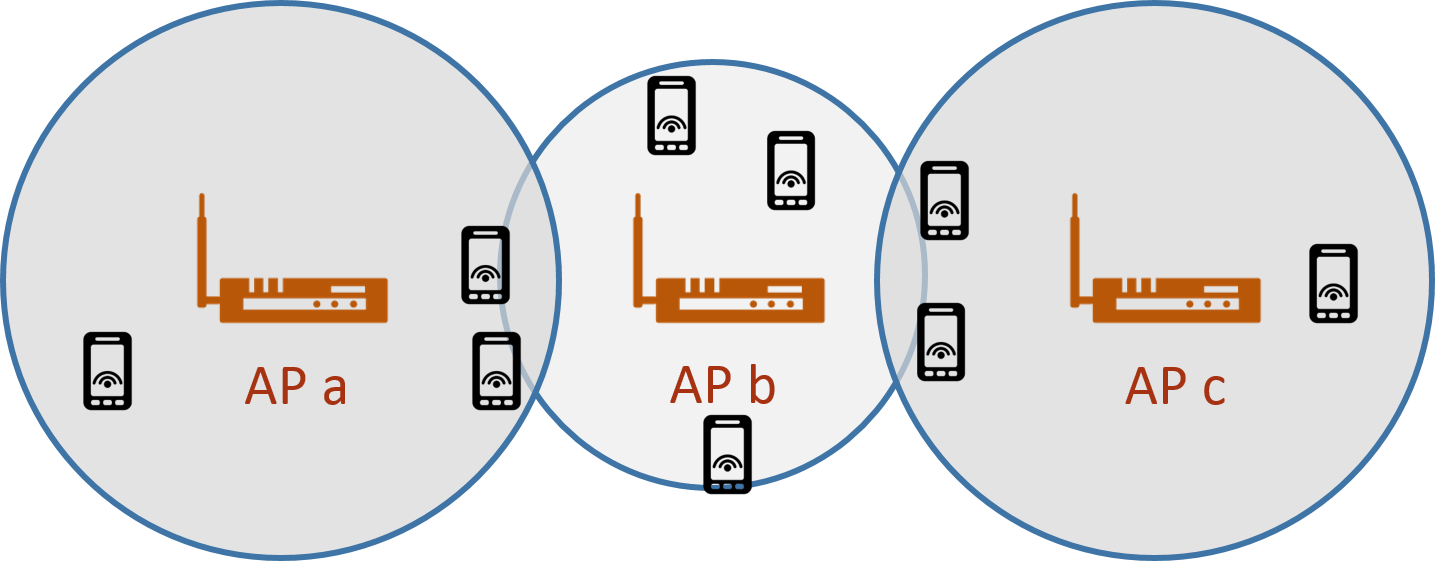
\includegraphics[scale=0.23]{images/cb_after.png}
			\label{fig:fig2_2b}
		}
		
	\caption{Using Cell Breathing Method for Imbalanced Situation.}
	\label{fig:cell-breathing}
\end{figure}

In this paper, we propose an adaptive load balancing scheme which can further improve performance of
%by combining the 
cell breathing by considering the flexibility of SDN.
% method with SDN. 
Through SDN, we can use the global vision to collect the load of AP and users' RSSIs accurately. 
%In this way, our scheme is adaptive. 
Furthermore, the users' positions can be derived by users' RSSI according to~\cite{zaruba2007indoor}. 
% above Dotto

